\documentclass[11pt]{article}
\usepackage{titlesec}
\usepackage{titling}
\usepackage{fontspec}
% Specify different font for section headings
\newfontfamily\headingfont[]{Gill Sans}
\titleformat*{\section}{\LARGE\headingfont}
\titleformat*{\subsection}{\Large\headingfont}
\titleformat*{\subsubsection}{\large\headingfont}
\renewcommand{\maketitlehooka}{\headingfont}

%\headheight=8pt
%\topmargin=3pt
%\textheight=624pt
%\textwidth=432pt
%\oddsidemargin=18pt
%\evensidemargin=18pt
\usepackage{amsmath}
\usepackage{amsfonts}
\usepackage{amssymb}
\usepackage{amsthm}
\usepackage{comment}
\usepackage{epsfig}
\usepackage{psfrag}
%\usepackage{sseq} (if you need to draw spectral sequences, please use this package, available at http://wwwmath.uni-muenster.de/u/tbauer/)
\usepackage{mathrsfs}
\usepackage{amscd}
\usepackage[all]{xy}
\usepackage{rotating}
\usepackage{lscape}
\usepackage{amsbsy}
\usepackage{verbatim}
\usepackage{moreverb}
\usepackage{mathdots}
\usepackage{setspace}
%\usepackage{eucal}
\usepackage{hyperref}

\usepackage{listings}
%\spacing{1.75}
\usepackage[margin=1in]{geometry}
\pagestyle{plain}
\theoremstyle{definition}
\newtheorem{theorem}{Theorem}%[section]
\newtheorem{prop}[theorem]{Proposition}
\newtheorem{lemma}[theorem]{Lemma}
\newtheorem{corollary}[theorem]{Corollary}
%\theoremstyle{definition}
\newtheorem{definition}[theorem]{Definition}
\newtheorem{notation}[theorem]{Notation}
\newtheorem{summary}[theorem]{Summary}
\newtheorem{note}[theorem]{Note}
\newtheorem{construction}[theorem]{Construction}
%\theoremstyle{remark}
\newtheorem{remark}[theorem]{Remark}
\newtheorem{example}[theorem]{Example}
\newtheorem{question}[theorem]{Question}
\DeclareMathOperator{\Aut}{Aut}
\DeclareMathOperator{\coeq}{coeq}
\DeclareMathOperator{\colim}{colim}
\DeclareMathOperator{\cone}{cone}
\DeclareMathOperator{\Der}{Der}
\DeclareMathOperator{\Ext}{Ext}
\DeclareMathOperator{\hocolim}{hocolim}
\DeclareMathOperator{\holim}{holim}
\DeclareMathOperator{\Hom}{Hom}
\DeclareMathOperator{\Iso}{Iso}
\DeclareMathOperator{\Map}{Map}
\DeclareMathOperator{\Tot}{Tot}
\DeclareMathOperator{\Tor}{Tor}
\DeclareMathOperator{\Spec}{Spec}
\newcommand{\TMF}{\mathit{TMF}}
\newcommand{\tmf}{\mathit{tmf}}
\newcommand{\Mell}{\mathcal M_{\mathit{ell}}}
\newcommand{\Mord}{\mathcal M_{\mathit{ell}}^{\mathit{ord}}}
\newcommand{\Mss}{\mathcal M_{\mathit{ell}}^{\mathit{ss}}}
\newcommand{\Mbar}{\overline{\mathcal M}_{\mathit{ell}}}
\newcommand{\Mfg}{\mathcal M_{\mathit{FGL}}}
\newcommand{\MU}{\mathit{MU}}
\newcommand{\MP}{\mathit{MP}}
\newcommand{\Lk}{L_{K(n)}}
\newcommand{\Lone}{L_{K(1)}}
\newcommand{\Ltwo}{L_{K(2)}}
\newcommand{\Sp}{\mathbf{Sp}}
\newcommand{\Eoo}{E_\infty}
\newcommand{\Aoo}{A_\infty}
\newcommand{\CP}{\mathbb{CP}^\infty}
\newcommand{\GL}{\mathit{GL}}
\newcommand{\gl}{\mathit{gl}}
\newcommand{\nn}{\nonumber}
\newcommand{\nid}{\noindent}
\newcommand{\ra}{\rightarrow}
\newcommand{\la}{\leftarrow}
\newcommand{\xra}{\xrightarrow}
\newcommand{\xla}{\xleftarrow}
\newcommand{\weq}{\xrightarrow{\sim}}
\newcommand{\cofib}{\rightarrowtail}
\newcommand{\fib}{\twoheadrightarrow}
\def\llarrow{   \hspace{.05cm}\mbox{\,\put(0,-2){$\leftarrow$}\put(0,2){$\leftarrow$}\hspace{.45cm}}}
\def\rrarrow{   \hspace{.05cm}\mbox{\,\put(0,-2){$\rightarrow$}\put(0,2){$\rightarrow$}\hspace{.45cm}}}
\def\lllarrow{  \hspace{.05cm}\mbox{\,\put(0,-3){$\leftarrow$}\put(0,1){$\leftarrow$}\put(0,5){$\leftarrow$}\hspace{.45cm}}}
\def\rrrarrow{  \hspace{.05cm}\mbox{\,\put(0,-3){$\rightarrow$}\put(0,1){$\rightarrow$}\put(0,5){$\rightarrow$}\hspace{.45cm}}}
\def\cA{\mathcal A}\def\cB{\mathcal B}\def\cc{\mathbf C}\def\cd{\mathbf D}
\def\ce{\mathcal E}\def\cf{\mathcal F}\def\cG{\mathcal G}\def\cH{\mathcal H}
\def\cI{\mathcal I}\def\cJ{\mathcal J}\def\cK{\mathcal K}\def\cL{\mathcal L}
\def\cM{\mathbf M}\def\cN{\mathcal N}\def\cO{\mathbf O}\def\cP{\mathcal P}
\def\cQ{\mathcal Q}\def\cR{\mathcal R}\def\cS{\mathcal S}\def\cT{\mathcal T}
\def\cU{\mathcal U}\def\cV{\mathcal V}\def\cW{\mathcal W}\def\cX{\mathcal X}
\def\cY{\mathcal Y}\def\cZ{\mathcal Z}
\def\AA{\mathbb A}\def\BB{\mathbb B}\def\CC{\mathbb C}\def\DD{\mathbb D}
\def\EE{\mathbb E}\def\FF{\mathbb F}\def\GG{\mathbb G}\def\HH{\mathbb H}
\def\II{\mathbb I}\def\JJ{\mathbb J}\def\KK{\mathbb K}\def\LL{\mathbb L}
\def\MM{\mathbb M}\def\NN{\mathbb N}\def\OO{\mathbb O}\def\PP{\mathbb P}
\def\QQ{\mathbb Q}\def\RR{\mathbb R}\def\SS{\mathbb S}\def\TT{\mathbb T}
\def\UU{\mathbb U}\def\VV{\mathbb V}\def\WW{\mathbb W}\def\XX{\mathbb X}
\def\YY{\mathbb Y}\def\ZZ{\mathbb Z}
%%%%%%%%%%%%%%%%
%%% Put individual commands and macros here.  Please also note in this section 
%%% if you had to alter the above existing commands and declarations in any way.
%%%%%%%%%%%%%%%%
\newcommand{\MFGL}{\mathcal M_{\mathit{FGL}}}
\newcommand{\calO}{{\mathcal O}}
\newcommand{\calC}{{\mathcal C}}
\newcommand{\set}{{\mathrm{Set}}}
\newcommand{\Deltab}{{\mathbf \Delta}}
\newcommand{\spet}{\mathrm{Spec}^\mathrm{\acute{e}t}}
\newcommand{\Z}{\mathbb Z}
\DeclareMathOperator{\Spf}{Spf}
%\usepackage{titlesec}
%\titleformat{\section}[runin]{\normalfont\bfseries}{\thesection. }{0em}{}
%\titleformat{\subsection}[runin]{\normalfont\bfseries}{\thesubsection. }{0em}{}
%\usepackage{ebgaramond}

\begin{document}
\title{Harker Advanced Topics in Mathematics: Information Theory
}
\author{Manan Shah}
\maketitle

This document contains lecture notes from Harker's Advanced Topics in Mathematics class in Information Theory, Part I. These notes were taken using TeXShop and \LaTeX2$\epsilon$, and will be updated for each class.
\section{Overview}
\begin{figure}
\centering
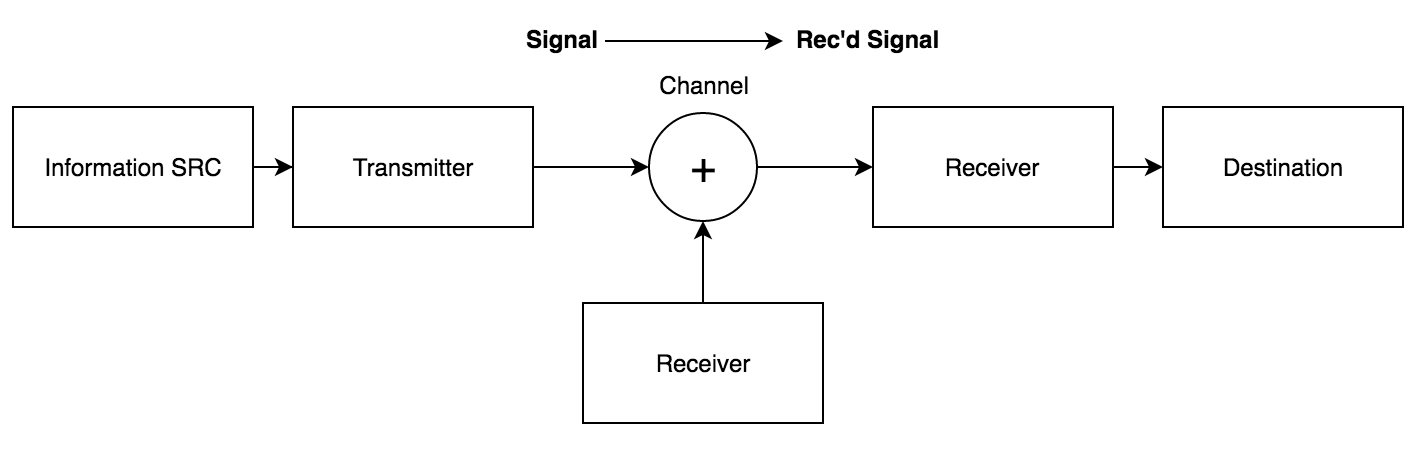
\includegraphics[scale=0.5]{pipeline}
\end{figure}
Information may be conveyed in multiple ways; for example, by a person talking, a video, or pictures. Our goal is to model this kind of information as a system with one output and no input. The information is therefore a box that emits output probabilistically, and we will therefore be spending 1-2 weeks on probability, specifically regarding distribution functions and expectation. This is illustrated in the ``information source'' box---the job of the information source is to \textbf{provide the signal}. 

We will next define the compression problem; having obtained numbers as a stream, the problem is to remove the redundancy in a stream. In particular, we will discuss both lossless and lossy compression. One of the most critical ideas in this course is that of entropy, and we will define the concept (in general, a notion of how much information is originating from the source). We will also discuss the sensibility of such a definition and potentially expand upon it. An overarching concept here will be our definition of the performance of a compression algorithm via the source compression theorem and the boundedness of compression algorithms. This is illustrated in the ``transmitter'' box---the job of the transmitter is to \textbf{remove all redundancy}.

We will subsequently discuss the channel circle, which we will model with conditional probability distribution functions (PDFs). The output of this box, the receiver signal, is input to the receiver box, which has the job of \textbf{reconstruction of the signal and the noise}; this is known as the coding problem. Much like the compression problem of the source, the channel has the capacity problem (how much information can be transmitted?). And similar to the compression theorem, we will discuss the channel coding theorem, which will help us determine which parts of a code will require more redundancy for transmission. 

We will finally discuss Shannon's theorem, in which he states that a communication with no loss and arbitrary cost (due to a constraint on the amount of bandwith, power, etc.) is possible if the entropy of the source $H$ is less than the capacity of the channel $C$. In our course, we will first discuss the pipeline for lossless compression and then move to lossy compression.

\end{document}
